%%*************************************************************************
%%
%% Anomaly detection by means of fourier tranform
%% V1.0
%% 2011/07/25
%% by Peter Boraros
%% See http://www.pborky.sk/contact for current contact information.
%%
%%*************************************************************************
%%
%% Legal Notice:
%%
%% This code is offered as-is without any warranty either expressed or
%% implied; without even the implied warranty of MERCHANTABILITY or
%% FITNESS FOR A PARTICULAR PURPOSE! 
%% User assumes all risk.
%%
%% This work by Peter Boraros is licensed under a 
%% Creative Commons Attribution-NonCommercial-ShareAlike 3.0 Unported License.
%% http://creativecommons.org/licenses/by-nc-sa/3.0/
%%
%%*************************************************************************

\documentclass[a4paper]{IEEEtran}

\usepackage{cite}
% \usepackage[nocompress]{cite}
\usepackage{ifpdf}

\ifpdf
\usepackage[pdftex]{graphicx}
\graphicspath{{./img/}}
\DeclareGraphicsExtensions{.pdf}
\else
\usepackage[dvips]{graphicx}
\graphicspath{{./img/}}
\DeclareGraphicsExtensions{.eps}
\fi

\usepackage[cmex10]{amsmath}
\usepackage{amsfonts}
\usepackage{amssymb}
\interdisplaylinepenalty=2500

\usepackage{algorithmic}

\usepackage{array}

\usepackage{mdwmath}
\usepackage{mdwtab}

\usepackage{eqparbox}

\usepackage[hang,small,center,bf]{caption}
% \usepackage[tight,normalsize,sf,SF]{subfigure}
%\usepackage[tight,footnotesize]{subfigure}
\usepackage{subfig}
% \usepackage[caption=false,font=normalsize,labelfont=sf,textfont=sf]{subfig}
% \usepackage[caption=false,font=footnotesize]{subfig}

\usepackage[utf8x]{inputenc}
\usepackage{url}
\usepackage{fixltx2e}
\usepackage{stfloats}
\usepackage{ucs}
\usepackage{multirow}

% correct bad hyphenation here
\hyphenation{op-tical net-works semi-conduc-tor}

\renewcommand{\labelitemi}{$\bullet$}
\renewcommand{\labelitemii}{$\circ$}
\renewcommand{\labelitemiii}{$\ast$}

\setlength{\textheight}{260mm}

\begin{document}
\title{Anomaly detection by means of fourier transform}
\date{July 25, 2011}
\author{Peter~Boraros %
\thanks{{Peter Boraros}, Czech technical university, Faculty of Electrical Engineering,
see~\texttt{http://www.pborky.sk/contact} for a contact infomation}}%

% The paper headers
\markboth{Peter Boraros, Czech technical university, Faculty of Electrical Engineering, Prague, Czech Republic}{}

\IEEEcompsoctitleabstractindextext{%
\begin{abstract}
The aim of this document is... 
\end{abstract}}

\maketitle
\IEEEdisplaynotcompsoctitleabstractindextext
\IEEEpeerreviewmaketitle

\section{Introduction}
This work provides explanation of the application of the Fourier transformation in terms of anomaly detection in computer network traffic.
Concretely it provides further desription in following topics:
\begin{itemize}
	\item data - detailed description of input vectors and process of theirs gathering;
	\item preprocessing - depicts the process of extracting features from the raw data in time domain;
	\item transformation of the features from the time domain to the frequency domain - fourier transformation has been used for the purposes of this work;
	\item normalisation and equalisation of the features - fits the data in the scale and evenly distributed;
	\item visualisation of the features - principal component analysis, displaying the kernel density estimator;
	\item clustering methods - grouping the ``similar'' features together;
	\item probabilistic aproach - ..
\end{itemize}

\section{Definitions}
\subsection{Network traffic, gathering the data}
Network traffic is set of flows distributed in time.
The flow is a sequence of packets, that has similar attributes. Packets
are exchanged usually among network endpoints. Attributes
under consderation are at least: source and destination endpoint address and port,
protocol. These are used to delimitate flows.

In order to evaluate anomaly rate of paticular flow other properties ought to be
taken in account. Especially number of packets and bytes, starting or ending time
(timestamp of the first or the last packet in the flow).

%TODO mention the features 
The time distribution of flows can be determined by considering the
starting timestamp of each flow. This approach provides generalized view on the flow, 
as it has been occured in network channel with unlimited throughput.

\subsection{Data binning}
In order to reduce minor observation errors binning technique ought to be used.
The time axis is divided into disjoint intervals - bins.
Let $n_\tau$ be number of bins and $F$ be the set of all flows captured in time interval
$T = (0, T_{max}\rangle $. The $\tau$-th bin is known as set of flows $F_\tau$ 
that occurs in time interval
$T_\tau = (\tau\cdot \delta, (\tau+1)\cdot \delta\rangle $ where 
$\tau \in \{0, 1, .. n_\tau-1\}$ and $\delta$ is the width of time intervals
denoted $\delta = \frac{T_{max}}{n_\tau}$.
Denote
\[
F_t = \{f : f \in F \wedge s(f) \in T_\tau \}
\]
where function $s:F \rightarrow N $ outputs starting timestamp of the flow $f\in F$.

For each interval,
representative value is calculated. Following formulas has been considered:
\[
r_\tau^{(1)} = \frac{\sum\limits_{f\in F_\tau}b(f)}{\sum\limits_{f\in F_\tau}p(f)}
\]
\[
r_\tau^{(2)} = \log(1+\sum\limits_{f\in F_\tau}b(f))
\]
where $r_\tau$ is representative of time interval $\tau$, $F_\tau$ is set of flows captured in time 
interval $\tau$, function $b:F \rightarrow N$ outputs size of the flow $f$ in bytes and function 
$p:F \rightarrow N$ outputs the packet count of the flow $f$.

%TODO further description of representatives

\subsection{Fourier transformation}

\section{Conclusion}
fooka

\section{Outline}
\subsection{Current state}
\begin{itemize}
	\item data - detailed explanation of the data for the experiment;
	\item preprocessing - describe the binning process and agregation of particular features; give explanation of what are the features meaning in context of network traffic;
	\item fourier transform - theory, contrast with wavelet transform;
	\item clustering methods (k-means, SOM);
	\item reducing the dimensionality - PCA, frequency filters;
	\item probabilistic aproach - kernel density estimator.
\end{itemize}
\subsection{Ideas}
\begin{itemize}
	\item compute probability density more accurately;
	\item transform the probability density to the fuzzy sets;
	\item more datasets are needed;
	\item 
\end{itemize}

%\begin{figure*}[!h] %
%  \centering
%  \subfloat[PCA projection]{\label{fig:som_topol_proj_7}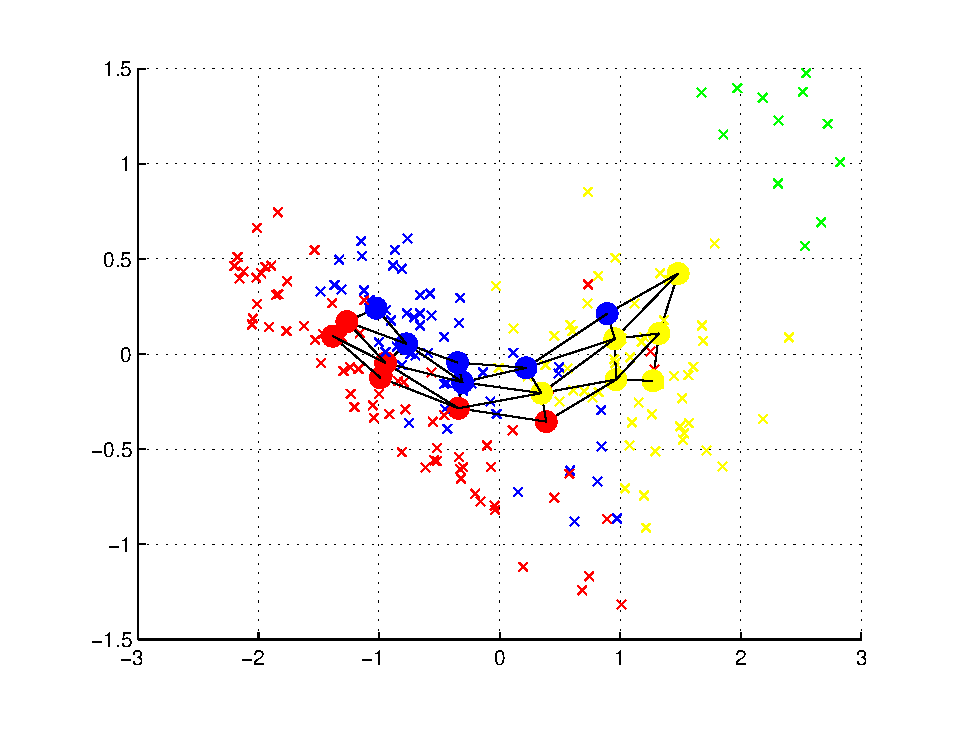
\includegraphics[width=55mm]{som_topol_proj_7}}
%  \subfloat[Sammon projection]{\label{fig:som_samon_proj_7}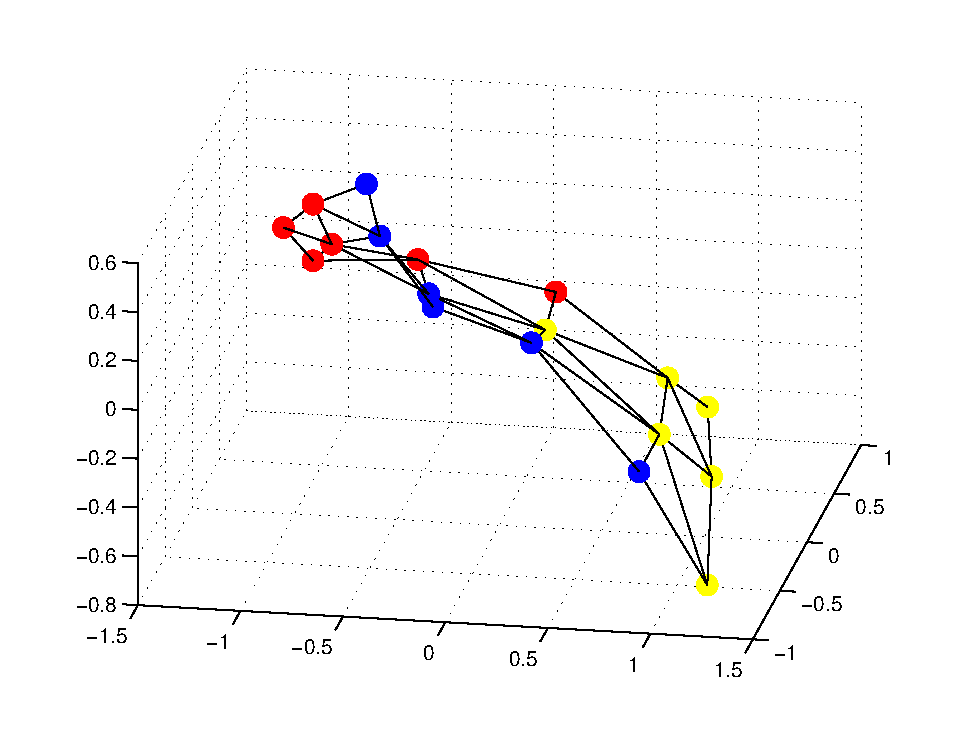
\includegraphics[width=55mm]{som_samon_proj_7}}
%  \subfloat[U-matrix and classification]{\label{fig:som_umat_7}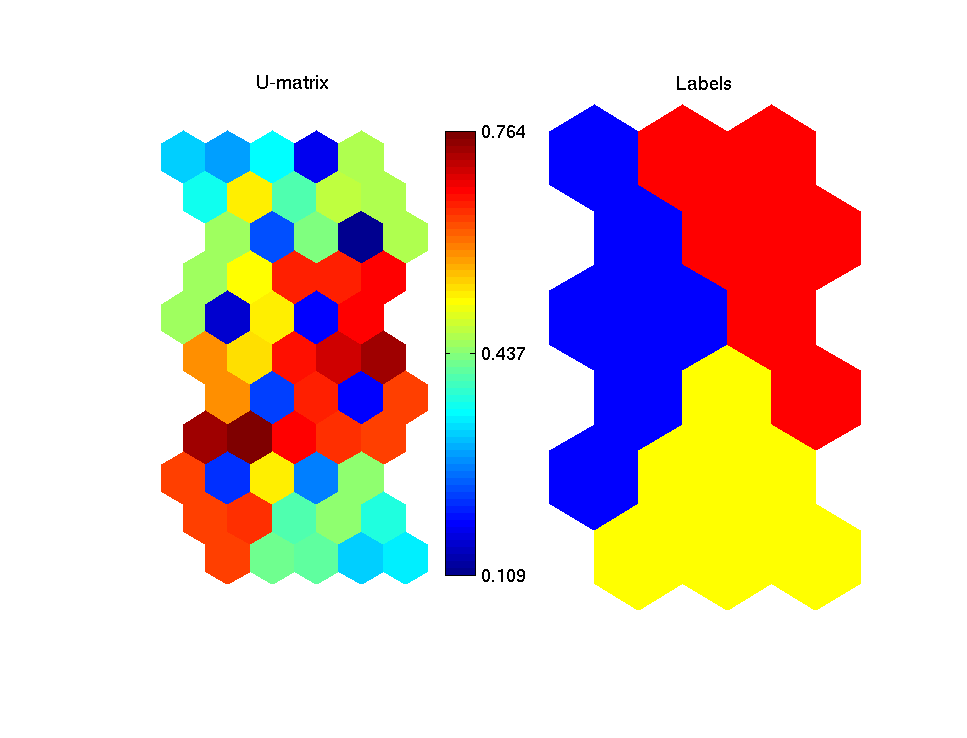
\includegraphics[width=55mm]{som_umat_7}}
%  \caption{configuration \#7 (see \textit{tbl. \ref{tbl:somresults}})}
%  \label{fig:som_config_7}
%\end{figure*}

% that's all folks
\end{document}
